\documentclass{tpm2026} % for initial submission
%\documentclass[accepted]{tpm2026} % after acceptance

\usepackage[american]{babel}
\usepackage{natbib} 
    \bibliographystyle{plainnat}
    \renewcommand{\bibsection}{\subsubsection*{References}}
\usepackage{mathtools} 
\usepackage{booktabs}
\usepackage{multirow}
\usepackage{stfloats}
\usepackage{graphicx}
\usepackage{amssymb,amsmath,amsfonts,amsthm}
\usepackage{mathrsfs}
\usepackage{algorithm, algpseudocode}
\usepackage[font={small,it},labelfont=bf]{caption}

\newtheorem{theorem}{Theorem}
\newtheorem{definition}{Definition}

\renewcommand{\dbltopfraction}{0.92}
\renewcommand{\textfraction}{0.05}

\title{Linear Independent Component Analysis via Optimal Transport Metric as Contrast\thanks{Code: \url{https://anonymous.4open.science/r/ot_in_linear_ica-3DBC}}}

% The standard author block has changed for TPM 2026 to provide
% more space for long author lists and allow for complex affiliations
\author[1,2]{\href{mailto:ashutosh.jha@student.uni-tuebingen.de?Subject=TPM 2026 Paper Inquiry}{Ashutosh~Jha}}
\author[1]{Simon~Buchholz}
\author[1,3]{Michel~Besserve}
\author[2]{Joachim~Grammig}

\affil[1]{%
    Empirical Inference Group\\
    Max Planck Institute for Intelligent Systems, T\"ubingen
}
\affil[2]{%
    Chair of Statistics, Econometrics and Empirical Economics\\
    University of T\"ubingen
}
\affil[3]{%
    Institute of Artificial Intelligence\\
    TU Braunschweig
}

\begin{document}
\maketitle

\begin{abstract}
Linear Independent Component Analysis (ICA) recovers mutually independent source signals from their linear mixtures.
Information theory links independence to maximal non-Gaussianity; classical algorithms replace this objective with proxy contrast functions, including negentropy approximations, fourth-order cumulants, and parametric log-likelihoods.
We propose OT-ICA, which measures non-Gaussianity using a true metric, the squared Wasserstein distance $W_2^2$ to a standard Gaussian, computable by quantile sorting without density estimation.
We prove that $W_2^2$ of any proper mixture of non-Gaussian sources lies strictly below the weighted sum of the individual component $W_2^2$ values, establishing a unique global maximum at pure source directions and ensuring the ICA optimization is well-posed.
OT-ICA outperforms proxy-based methods on continuous and heterogeneous source distributions; on purely discrete sources, step-function CDFs produce gradient plateaus that hinder convergence, an open optimization problem.
Real-data applications to EEG artifact removal and econometric price discovery confirm transfer without distributional assumptions.
\end{abstract}

\section{Introduction}
Independent Component Analysis (ICA) \citep{jutten1985, comon1994} recovers mutually independent source signals $\mathbf{S}$ from 
a linear mixture $\mathbf{X} = \mathbf{A}\mathbf{S}$. Identifiability holds under the following conditions \citep{comon1994}.

\begin{theorem}[Linear ICA Identifiability]
Let $\mathbf{X} \in \mathbb{R}^d$ be observed data and $\mathbf{S} \in \mathbb{R}^d$ latent sources. 
Assume (i) $\mathbf{X} = \mathbf{A}\mathbf{S}$ with $\mathbf{A}$ invertible, (ii) $s_1, \dots, s_d$ are mutually independent, 
and (iii) at most one $s_i$ Gaussian. Then $\mathbf{A}$ is identifiable up to column permutation and scaling.
\end{theorem}

The Central Limit Theorem implies that linear mixtures of independent non-Gaussian sources are more Gaussian than their constituents \citep{hyvarinen2001}.
Centering and whitening $\mathbf{X}$ to $\widetilde{\mathbf{X}}$ ($\mathbb{E}[\widetilde{\mathbf{X}}] = \mathbf{0}$, $\operatorname{Cov}[\widetilde{\mathbf{X}}] = \mathbf{I}$) reduces the full $d^2$-parameter search over invertible
mixing matrices to a search over the compact Orthogonal Group $\mathrm{O}(d)$ (the set of $d\times d$ real matrices satisfying $\mathbf{B}\mathbf{B}^\top = \mathbf{I}$).
This preprocessing is lossless for identifiable ICA (Appendix~\ref{app:info_geometry}).
ICA recovers sources by maximizing marginal non-Gaussianity over Orthogonal Group $\mathrm{O}(d)$ \citep{hyvarinen2001}, justified by the following identity, further details in Appendix~\ref{app:info_geometry}.

\begin{theorem}[Independence and Non-Gaussianity \citep{cardoso2022}]
Let $Y \in \mathbb{R}^d$ be whitened ($\operatorname{Cov}(Y)=\mathbf{I}$). The mutual information $\mathscr{I}(Y)$, which measures statistical dependence among components $Y_1,\ldots,Y_d$, satisfies:
\begin{equation}
    \mathscr{I}(Y) = G(Y) - \sum_{i} G(Y_i)
\end{equation}
where $G(\cdot)$ denotes non-Gaussianity (KL divergence to the best-fitting Gaussian). Since $G(Y)$ is invariant under orthogonal rotation,
minimizing $\mathscr{I}(Y)$ towards independence is equivalent to maximizing total marginal non-Gaussianity $\sum_i G(Y_i)$.
\end{theorem}

Evaluating $G(Y_i)$ requires the marginal density. Classical algorithms replace it with proxy contrasts:
FastICA \citep{hyvarinen2001, amari1996new} uses logcosh negentropy approximations, 
JADE \citep{cardoso1993blind} fourth-order cumulants, 
InfoMax \citep{bell1995information} a parametric log-likelihood, and 
Picard \citep{ablin2018faster} an adaptive nonlinearity with a provably converging solver. 
Each proxy fails on specific source geometries (Appendix~\ref{app:proxy_limits}).

We propose OT-ICA, using the squared Wasserstein distance $W_2^2$ to a standard Gaussian as the contrast. Unlike proxy contrasts, Optimal Transport \citep{monge1781, kantorovich1942}
provides a true metric on the space of probability distributions,
quantifying non-Gaussianity as the cost of transporting the empirical projection to a fixed standard Gaussian reference (Appendix~\ref{app:info_geometry}). The $p$-Wasserstein distance ($L_2$ for $p=2$) \citep{villani2003} is the minimum-cost coupling:
\begin{equation}
    W_p(\mu, \nu) = \left( \inf_{\pi \in \Pi(\mu, \nu)} \int \|x - y\|^p \, d\pi(x, y) \right)^{1/p}
\end{equation}
In 1D, Brenier's theorem \citep{brenier1991} and Caffarelli's regularity \citep{caffarelli1992} guarantee that the optimal map is monotone, reducing $W_2^2$ to:
\begin{equation}
    W_2^2(\mu, \nu) = \int_0^1 |F_\mu^{-1}(t) - F_\nu^{-1}(t)|^2 \, dt
\end{equation}
This is computable by quantile sorting. Prior work uses 1D $W_2$ for normality testing \citep{delbarrio1999} and 
distribution comparison \citep{peyre2019computational}; we formalize $W_2^2$ distance to Gaussian as a valid ICA contrast with finite-sample convergence guarantees.

\section{The OT-ICA Framework}

After centering and whitening $\mathbf{X}$ to $\widetilde{\mathbf{X}}$, 
the unmixing matrix is constrained to Orthogonal Group $\mathrm{O}(d)$ \citep{cardoso2022}.
OT-ICA finds the projection $\mathbf{b}$ maximizing $W_2^2$ to the standard Gaussian $\Gamma \equiv \mathcal{N}(0,1)$:
\begin{equation}
    \hat{\mathbf{b}} = \arg\max_{\mathbf{b} \in \mathrm{O}(d)} W_2^2\big(\mathbb{P}_{\mathbf{b}^\top \widetilde{\mathbf{X}}}, \Gamma\big).
\end{equation}

The following theorem ensures the optimization in Eq.~(3) is well-posed: any proper mixture of non-Gaussian sources yields a $W_2^2$ value below that of its most non-Gaussian component, so the maximum is uniquely attained at pure source directions.

\begin{theorem}[$W_2^2$ ICA Contrast]
Let $\mathbf{Z} = (Z_1, \dots, Z_d)^\top$ be mutually independent sources with at most one Gaussian, each having a smooth and strictly positive density. For any unit-sphere weight vector $\mathbf{b}$ with at least two nonzero components:
\begin{equation}
    W_2^2(\mathbf{b} \cdot \mathbf{Z}, \Gamma) < \sum_{i=1}^d b_i^2 W_2^2(Z_i, \Gamma).
\end{equation}
\end{theorem}

Since equality holds trivially when $\mathbf{b} = \mathbf{e}_k$ (a pure source direction), the global maximum of Eq.~(3) is uniquely attained at source directions (Appendix~\ref{app:proofs}).

\subsection{Optimization on Orthogonal Group $\mathrm{O}(d)$}
Independent components are mutually orthogonal in the whitened space, which restricts the search: each source direction must lie in the orthogonal complement of the already-found directions.
One can exploit this iteratively, extracting one component at a time from the shrinking complement.
In practice we implement this as symmetric joint optimization: all $d$ rows of $\mathbf{B}$ are updated simultaneously under the $\mathrm{O}(d)$ constraint via symmetric decorrelation retraction, so mutual orthogonality is maintained at every step rather than enforced by sequential projection, eliminating error accumulation across components (Appendix~\ref{app:methodology}).
Three algorithmic components are required: (i)~\textbf{Analytical Gaussian Targets} \citep{fournier2015rate}, replacing sampled quantile targets with closed-form bin expectations to eliminate approximation noise; (ii)~\textbf{Riemannian Gradient Retraction} \citep{absil2008optimization}, projecting gradients onto the tangent space of Orthogonal Group $\mathrm{O}(d)$ and retracting via symmetric decorrelation (Newton updates are intractable for empirical OT; Appendix~\ref{app:intractability}); and (iii)~\textbf{Gaussian Dithering} \citep{schuchman1964dither}, smoothing discrete CDFs via narrow Gaussian convolution.

\section{OT-ICA Methodology Validation}
Separation quality is measured by the Amari Performance Index ($E$) \citep{amari1996new}, 
the deviation of the gain matrix $\mathbf{P} = \mathbf{B}_{\text{est}}\mathbf{A}$ from a 
generalized permutation matrix ($E < 0.1$: near-perfect; $E < 0.3$: good separation; $E \ge 0.5$: failure; definition in Appendix~\ref{app:experimental_setup}).

\begin{figure}[h]
    \centering
    
\includegraphics[width=0.95\columnwidth]{otica_baseline_recovery.pdf}
    \caption{OT-ICA convergence on four standard continuous source types. $W_2^2$ provides a smooth contrast that drives the Amari error to near zero across optimization iterations.}
    \label{fig:ot_ica_validation}
\end{figure}

Figure~\ref{fig:ot_ica_validation} shows $W_2^2$ driving the Amari error to near zero on Laplace, Uniform, Student-$t$, and Beta sources,
confirming convergence on continuous distributions; OT-ICA achieves $E = 0.016$ against FastICA's $0.019$ on this 4D mixture
(Table~\ref{tab:baseline_matrices}, Appendix~\ref{app:experimental_setup}).

\begin{figure*}[!b]
    \centering
    
\includegraphics[width=0.88\textwidth]{general_hybrid_test.pdf}
    \caption{Mean Amari error ($\downarrow$ better, clipped at $1.5$) across five mixture regimes and $d \in \{10, 20, 30\}$ ($N=10{,}000$, 10 trials, 95\% CI). OT-ICA achieves the lowest error on all continuous and heterogeneous regimes at every dimension. On \textit{Discrete Only}, step-function CDFs produce gradient plateaus that stall the solver despite a present $W_2^2$ signal (Appendix~\ref{app:discrete_contrast}); at $d=30$ all methods saturate the clip ceiling. Dotted line marks $E=0.3$, the good-separation threshold.}
    \label{fig:hybrid_mixture_results}
\end{figure*}

\section{Empirical Performance on Heterogeneous Mixtures}
\label{sec:empirical}

We compare OT-ICA against FastICA \citep{hyvarinen2001}, JADE \citep{cardoso1993blind}, InfoMax \citep{bell1995information}, and 
Picard \citep{ablin2018faster} on five mixture regimes at $d \in \{10, 20, 30\}$, $N = 10{,}000$, 10 trials per condition (Figure~\ref{fig:hybrid_mixture_results}).

\textbf{Continuous and heterogeneous regimes.} OT-ICA achieves the lowest Amari error on all four continuous and mixed-type configurations at every dimension (Table~\ref{tab:full_amari_results}, Appendix~\ref{app:experimental_setup}). On \textit{Continuous Only} sources, OT-ICA reduces error $40$--$45\%$ over FastICA across all three dimensions. The margin is larger on \textit{Full Hybrid} mixtures (Laplace, Gaussian, Uniform, Student-$t$, Beta combined): OT-ICA attains $E = 0.059$, $0.261$, $0.335$ at $d = 10, 20, 30$ against FastICA's $0.255$, $0.451$, $0.671$, a factor of $2$--$4\times$. On \textit{Zero Gaussian} sources, OT-ICA outperforms InfoMax, which is misspecified for that mixture type, by a similar margin at all dimensions.

\textbf{Discrete sources.} On Discrete Only mixtures, OT-ICA underperforms JADE at $d = 10$ ($0.706$ vs.\ $0.443$) and $d = 20$ ($1.331$ vs.\ $1.267$); note both values exceed $E = 0.5$, placing all methods in failure territory where differences reflect degree of failure rather than separation quality (a $d$-dimensional random orthogonal matrix yields $E \approx (d-1)/d$, e.g.\ $\approx 0.97$ at $d=30$; Appendix~\ref{app:experimental_setup}). At $d = 30$ all methods including OT-ICA saturate the clip ceiling ($1.500$). Table~\ref{tab:w2_sensitivity} shows $W_2^2$ retains a clear non-Gaussianity signal on count data, exceeding logcosh resolution by more than $10{\times}$ on standard Poisson($\lambda=3$), so the failure is not a contrast deficiency. Step-function CDFs create gradient plateaus that stall the Riemannian solver despite the contrast being non-zero (Appendix~\ref{app:discrete_contrast}). Gaussian dithering (Appendix~\ref{app:methodology}) smooths CDF steps but does not fully restore the gradient signal at these scales.

\textbf{Baseline comparisons.} FastICA and Picard \citep{ablin2018faster} produce nearly identical errors across all configurations (within $0.003$), confirming the shared tanh nonlinearity, not the solver, as the bottleneck; replacing it with $W_2^2$ yields the $40$--$45\%$ error reduction on continuous sources. JADE requires $\mathcal{O}(d^4)$ samples (${\approx}810{,}000$ at $d=30$ vs.\ $N=10{,}000$ available), yielding $E=0.489$ on continuous and $0.938$ on hybrid at $d=30$; InfoMax is misspecified on mixed super- and sub-Gaussian components, producing $E=0.765$ on hybrid at $d=30$ against OT-ICA's $0.335$ (Appendix~\ref{app:proxy_limits}).

OT-ICA's gradient-based Riemannian solver requires more time than FastICA's fixed-point Newton iterations, with the gap widening as $d$ increases; 
this cost is offset on heterogeneous mixtures where proxy methods fail to separate independent sources  (Appendix~\ref{app:scaling}).

\section{Interdisciplinary Applications}

\subsection{Structural Identification in Price Discovery}
In fragmented financial markets, the Information Share (IS) \citep{hasbrouck1995, baillie2002} quantifies each venue's contribution to price discovery from the structural decomposition $u_t = \mathbf{B}\epsilon_t$, with $u_t$ the VECM reduced-form residuals and $\epsilon_t$ structural innovations \citep{engle1987, johansen1991}. The covariance constraint $\boldsymbol{\Omega} = \mathbf{B}\mathbf{B}^\top$ leaves $\mathbf{B}$ unidentified up to an orthogonal rotation; Cholesky identification depends on an arbitrary market ordering. Factoring $\mathbf{B} = \mathbf{S}\mathbf{C}$ \citep{zema2025} reduces identification to finding $\mathbf{C}$, which OT-ICA recovers from the non-Gaussianity of innovations without ordering assumptions.
We validate on a simulated three-market VECM \citep{zema2025}: $\mathbf{B}_\text{true} = \mathrm{diag}(\sqrt{0.12}, \sqrt{0.24}, \sqrt{0.64})$ encodes true IS values $[0.12, 0.24, 0.64]$ by construction, with Student-$t$ innovations enabling ICA identification.
IS estimates match true values to within $0.002$ across 500 Monte Carlo runs (Table~\ref{tab:simulated_is_results}, Appendix~\ref{app:price_discovery}).

\begin{table}[htbp]
    \centering
    \resizebox{\columnwidth}{!}{
    \begin{tabular}{@{}lccc@{}}
        \toprule
        \textbf{Market / Source} & \textbf{True IS} & \textbf{Estimated IS (Mean)} & \textbf{Std. Dev.} \\
        \midrule
        Market 1 & 0.1200 & 0.1212 & 0.0161 \\
        Market 2 & 0.2400 & 0.2399 & 0.0245 \\
        Market 3 & 0.6400 & 0.6389 & 0.0260 \\
        \bottomrule
    \end{tabular}
    }
    \caption{IS recovery across 500 Monte Carlo runs without imposing Cholesky ordering.}
    \label{tab:simulated_is_results}
\end{table}

\subsection{EEG Artifact Removal}
The skull acts as a linear volume conductor \citep{hyvarinen2001}: ocular blink artifacts mix with neural signals before reaching scalp electrodes. 
Blink artifacts are impulsive and super-Gaussian; their high $W_2^2$ separates them from neural components without specifying a density model (dataset, preprocessing, and configuration in Appendix~\ref{app:eeg}).

\begin{figure}[t]
    \centering
    
\includegraphics[width=0.90\columnwidth]{eeg_artifact_removal.pdf}
    \caption{OT-ICA on five frontal EEG channels (MNE sample dataset). Panel (b): isolated blink component (orange) with 
    excess kurtosis $\kappa$ in the panel title; remaining components have mean $\kappa$ near zero. Panel (c): 
    signal reconstructed by zeroing the artifact component, with RMS reduction in the $\pm$250\,ms blink window in the panel title.}
    \label{fig:eeg_artifact}
\end{figure}

Figure~\ref{fig:eeg_artifact} shows OT-ICA concentrating the blink artifact into a single component with excess kurtosis 
substantially above the remaining four. Zeroing that component and inverting the total unmixing matrix produces 
the RMS reduction quantified in the panel title, without tuning a density model.

\section{Conclusion}
OT-ICA replaces proxy contrast functions with the true $W_2^2$ metric computed by quantile sorting, outperforming all proxy-based baselines on continuous and heterogeneous source distributions across every dimension tested; the Picard comparison isolates the contrast, not the solver, as the binding constraint. On purely discrete sources, all methods fail as $d$ increases ($E > 0.3$); for OT-ICA the $W_2^2$ contrast retains signal throughout but step-function CDFs stall the solver, an open optimization problem. OT-ICA's higher per-iteration cost grows with $d$ (Appendix~\ref{app:scaling}) but is offset by superior separation quality on heterogeneous mixtures where proxy methods fail.
Applications to VECM structural identification and EEG artifact removal confirm transfer to real data without distributional assumptions.
Future work will extend OT-ICA to causal discovery as a front-end for LiNGAM \citep{shimizu2006linear}, Causal Component Analysis \citep{liang2023causal}, and identifiable nonlinear ICA \citep{buchholz2022function}.

\newpage
\bibliography{references}

\newpage
\onecolumn
\appendix

\begin{center}
    \Large\textbf{Supplementary Material for:}\\
    \large\textbf{Linear Independent Component Analysis via Optimal Transport Metric as Contrast}
\end{center}

\section{Background and Motivation}
\label{app:info_geometry}

\subsection{Centering, Whitening, and the Orthogonal Group $\mathrm{O}(d)$ Search Space}

The ICA model $\mathbf{X} = \mathbf{A}\mathbf{S}$ has $d^2$ free parameters in the mixing matrix $\mathbf{A}$.
Two lossless preprocessing steps reduce this to a $\tfrac{d(d-1)}{2}$-dimensional rotational search.

\textbf{Centering.} Subtracting the mean, $\mathbf{X} \gets \mathbf{X} - \mathbb{E}[\mathbf{X}]$, ensures the data has zero mean.
If $\mathbf{X} = \mathbf{A}\mathbf{S}$, centering $\mathbf{X}$ is equivalent to centering $\mathbf{S}$, leaving the mixing geometry intact.

\textbf{Whitening.} Given the eigendecomposition $\mathrm{Cov}(\mathbf{X}) = \mathbf{V}\boldsymbol{\Lambda}\mathbf{V}^\top$, the whitening transform $\mathbf{Q} = \boldsymbol{\Lambda}^{-1/2}\mathbf{V}^\top$ yields $\widetilde{\mathbf{X}} = \mathbf{Q}\mathbf{X}$ with $\mathrm{Cov}(\widetilde{\mathbf{X}}) = \mathbf{I}$ \citep{hyvarinen2001}.
After whitening, the unmixing operation $\mathbf{B}\widetilde{\mathbf{X}}$ must satisfy $\mathrm{Cov}(\mathbf{B}\widetilde{\mathbf{X}}) = \mathbf{B}\mathbf{B}^\top = \mathbf{I}$, so $\mathbf{B}$ lies in Orthogonal Group $\mathrm{O}(d)$.
The original mixing matrix decomposes as $\mathbf{A} = \mathbf{Q}^{-1}\mathbf{B}$, so ICA on whitened data is lossless \citep{cardoso2022}.

\subsection{The CLT Motivation for Non-Gaussianity}

The Central Limit Theorem (CLT) provides the intuition: a normalized sum of independent non-Gaussian variables converges to a Gaussian as the number of terms grows \citep{hyvarinen2001}. In ICA, any linear mixture $\mathbf{b}\cdot\mathbf{S}$ with multiple nonzero weights is therefore \emph{more} Gaussian than the individual sources. Recovering an independent source means finding the projection that is \emph{least} Gaussian, motivating the maximization of non-Gaussianity as the ICA objective.

\subsection{Information Geometry: Connecting Independence and Non-Gaussianity}

Following \citet{cardoso2022}, ICA can be understood geometrically via two Pythagorean identities.
Let $G(\cdot) = D_{\mathrm{KL}}(\cdot \,\|\, \mathcal{N}(\mathrm{Cov}\,\cdot))$ denote non-Gaussianity and $C(Y) = D_{\mathrm{KL}}(\mathcal{N}(\mathrm{Cov}\,Y) \,\|\, \mathcal{N}(\mathrm{diag\,Cov}\,Y))$ denote correlation.

\textbf{Product manifold identity.} For any product distribution $Q = \prod_i q_i$:
\begin{equation}
    D_{\mathrm{KL}}(P_Y \Vert Q) = \mathscr{I}(Y) + \sum_{i} D_{\mathrm{KL}}(P_{Y_i} \Vert q_i).
\end{equation}

\textbf{Gaussian manifold identity.} For any Gaussian $\mathcal{N}(\Sigma)$:
\begin{equation}
    D_{\mathrm{KL}}(P_Y \Vert \mathcal{N}(\Sigma)) = G(Y) + D_{\mathrm{KL}}(\mathcal{N}(\mathrm{Cov}\,Y) \Vert \mathcal{N}(\Sigma)).
\end{equation}

Evaluating the KL divergence from $P_Y$ to $\mathcal{N}(\mathrm{diag\,Cov}\,Y)$ via both paths yields Cardoso's identity:
\begin{equation}
    \mathscr{I}(Y) + \sum_{i} G(Y_i) = G(Y) + C(Y).
\end{equation}
After whitening, $\mathrm{Cov}(Y) = \mathbf{I}$ forces $C(Y) = 0$, giving $\mathscr{I}(Y) = G(Y) - \sum_i G(Y_i)$.
Since $G(Y)$ is invariant under orthogonal rotation, minimizing $\mathscr{I}(Y)$ (independence) equals maximizing $\sum_i G(Y_i)$ (total marginal non-Gaussianity). This is Theorem 2. Figure~\ref{fig:cardoso_geometry} illustrates this Pythagorean geometry \citep{cardoso2022}.

\begin{figure}[htbp]
    \centering
    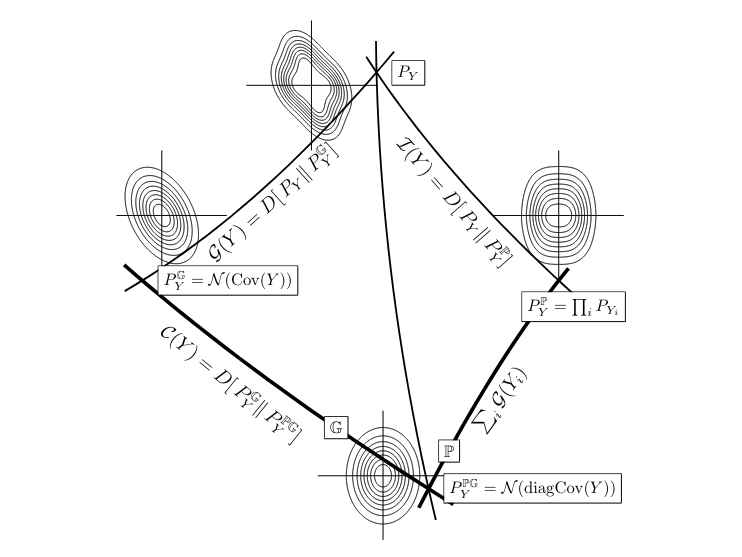
\includegraphics[width=0.75\textwidth]{pythagorean_ig_ica.png}
    \caption{The Pythagorean geometry of ICA. Figure from \citet{cardoso2022}.}
    \label{fig:cardoso_geometry}
\end{figure}

\subsection{Optimal Transport as the Non-Gaussianity Contrast}

Classical ICA algorithms approximate $G(Y_i)$ with proxies. OT-ICA instead measures it directly as the cost of transporting the empirical marginal to a standard Gaussian.

\begin{definition}[Coupling and Push-Forward]
A \emph{coupling} of distributions $\mu$ and $\nu$ is a joint distribution $\pi$ on $\mathbb{R}^d \times \mathbb{R}^d$ with marginals $\mu$ and $\nu$; the set of all such couplings is $\Pi(\mu,\nu)$.
A measurable map $T\colon\mathbb{R}^d\to\mathbb{R}^d$ \emph{pushes forward} $\mu$ to $\nu$ (written $T_\#\mu = \nu$) if $\nu(B) = \mu(T^{-1}(B))$ for every Borel set $B$.
\end{definition}

The $p$-Wasserstein distance is the minimum transport cost over all couplings:
\begin{equation}
    W_p(\mu,\nu) = \left(\inf_{\pi\in\Pi(\mu,\nu)} \int \|x-y\|^p\,d\pi(x,y)\right)^{1/p}.
\end{equation}
In 1D, Brenier's theorem guarantees the optimal coupling is induced by the monotone quantile map $T = F_\nu^{-1}\circ F_\mu$, so $W_2^2(\mu,\nu) = \int_0^1 |F_\mu^{-1}(t) - F_\nu^{-1}(t)|^2\,dt$.

\begin{figure}[htbp]
    \centering
    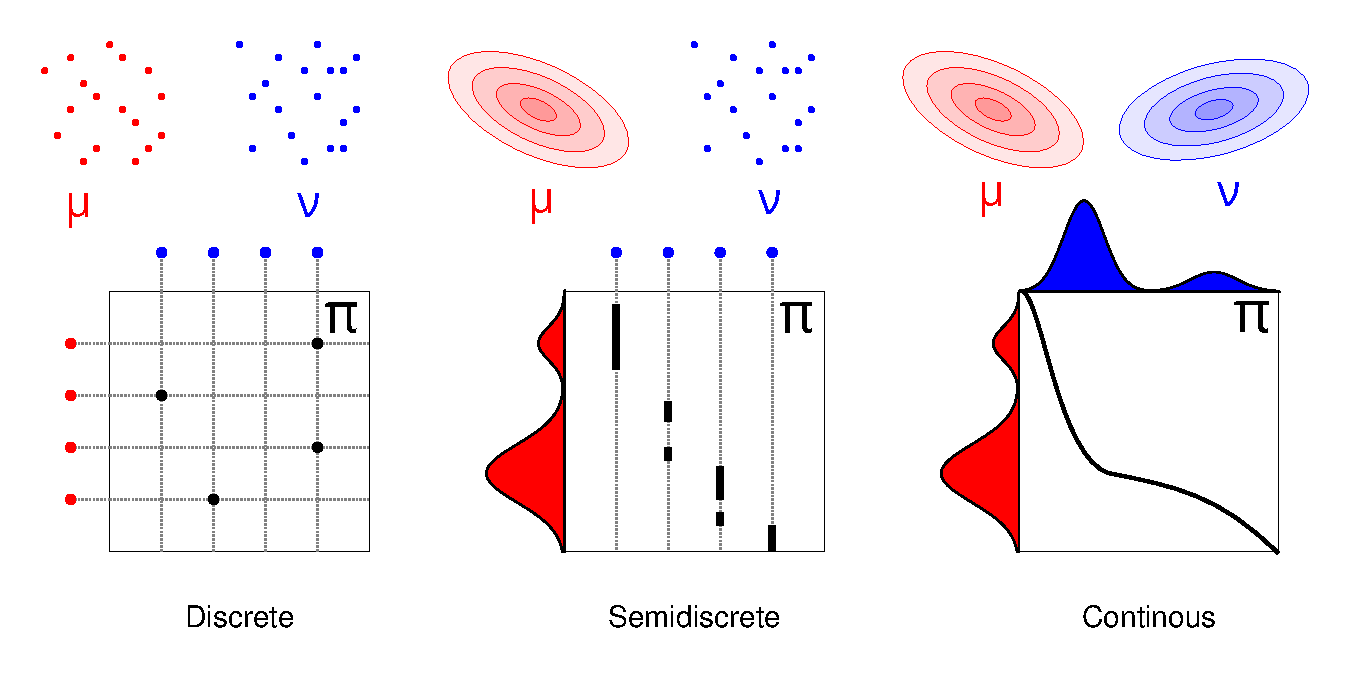
\includegraphics[width=0.85\textwidth]{ot_coupling_cases.pdf}
    \caption{Three coupling strategies between an empirical source distribution and the standard Gaussian $\Gamma$: arbitrary coupling (left), independent coupling (center), and the optimal monotone coupling that achieves $W_2^2$ (right).}
    \label{fig:ot_coupling}
\end{figure}

Taking $\nu = \Gamma \equiv \mathcal{N}(0,1)$, the quantity $W_2^2(\mathbb{P}_{\mathbf{b}^\top\widetilde{\mathbf{X}}},\Gamma)$ measures how far the projection $\mathbf{b}^\top\widetilde{\mathbf{X}}$ is from Gaussian.
Unlike negentropy proxies, $W_2^2$ is a true metric, geometry-aware, and computable by sorting without density estimation.
OT-ICA maximizes this over $\mathbf{b}$ in Orthogonal Group $\mathrm{O}(d)$; Theorem 3 shows the maximum is attained at pure source directions.

\section{Mathematical Proofs for OT-ICA Bounds}
\label{app:proofs}

\subsection{Proof of Theorem 3: $W_2^2$ ICA Contrast}

\setcounter{theorem}{2}
\begin{theorem}[$W_2^2$ ICA Contrast]
Let $\mathbf{Z} = (Z_1, \dots, Z_d)^\top$ be mutually independent sources with at most one Gaussian, each having a smooth and strictly positive density. For any unit-sphere weight vector $\mathbf{b}$ with at least two nonzero components:
\begin{equation}
    W_2^2(\mathbf{b} \cdot \mathbf{Z}, \Gamma) < \sum_{i=1}^d b_i^2 W_2^2(Z_i, \Gamma).
\end{equation}
\end{theorem}

\textit{Strategy.} We first establish a weak upper bound on $W_2^2(\mathbf{b}\cdot\mathbf{Z},\Gamma)$ (used as an intermediate step), then show the bound is strict for any proper mixture under the non-Gaussianity conditions, proving Theorem 3.

\medskip\noindent\textit{Step 1: Upper Bound (intermediate).}

\textit{Proof.} We construct a specific joint probability distribution, or coupling, using a common source of randomness. 
Let $\mathbf{N} = (N_1, \dots, N_d)^\top$ be a vector of $d$ independent standard normal variables, $\mathbf{N} \sim \mathcal{N}(0, \mathbf{I}_d)$, 
assumed to be statistically independent of the sources $\mathbf{Z}$. For each independent latent source $Z_i$, there exists 
an optimal transport map $T_i$ that pushes forward the standard normal distribution to the source distribution, denoted as $(T_i)_{\#} \Gamma = Z_i$. 

We construct a random variable $X$ representing the mixture:
\begin{equation}
    X = \sum_{i=1}^d b_i T_i(N_i).
\end{equation}
To compare this mixture to a Gaussian distribution, we construct a target variable $Y$ using the same underlying noise vector $\mathbf{N}$:
\begin{equation}
    Y = \sum_{i=1}^d b_i N_i.
\end{equation}
Given that the weights sum to unity, the resulting variable $Y$ follows the standard normal distribution, $Y \sim \Gamma$. 
The pair $(X, Y)$ creates a valid coupling. Because $W_2^2$ is the infimum over all valid couplings, the optimal distance is less than or equal to the cost of our constructed coupling:
\begin{equation}
    W_2^2(\mathbf{b} \cdot \mathbf{Z}, \Gamma) \le \mathbb{E}\left[|X - Y|^2\right] = \mathbb{E}\left[ \left( \sum_{i=1}^d b_i \big(T_i(N_i) - N_i\big) \right)^2 \right].
\end{equation}
Squaring the summation produces diagonal terms ($i=j$) and cross terms ($i \neq j$):
\begin{equation}
    |X - Y|^2 = \sum_{i=1}^d b_i^2 \big(T_i(N_i) - N_i\big)^2 + \sum_{i \neq j} b_i b_j \big(T_i(N_i) - N_i\big)\big(T_j(N_j) - N_j\big).
\end{equation}
Because the underlying noise variables $N_i$ and $N_j$ are independent, and the functions evaluate to a mean of zero, when we take the expectation, 
all cross terms vanish. We are left with the expectation of the diagonal terms:
\begin{equation}
    \mathbb{E}\left[|X - Y|^2\right] = \sum_{i=1}^d b_i^2 \mathbb{E}\left[ \big(T_i(N_i) - N_i\big)^2 \right].
\end{equation}
Recognizing that $\mathbb{E}[ (T_i(N_i) - N_i)^2 ]$ is the definition of the squared Wasserstein distance between the individual source $Z_i$ and $\Gamma$, we arrive at the bound:
\begin{equation}
    W_2^2(\mathbf{b} \cdot \mathbf{Z}, \Gamma) \le \sum_{i=1}^d b_i^2 W_2^2(Z_i, \Gamma). \quad \blacksquare
\end{equation}

\medskip\noindent\textit{Step 2: Strict Inequality (proof of Theorem 3).}
In a one-dimensional setting, the $W_2$ distance equals the expected squared difference of a specific coupling 
if and only if the random variables are comonotonic. By Brenier's Theorem \citep{brenier1991}, this requires the gradients 
to be parallel at every point in the probability space:
\begin{equation}
    \nabla X(\mathbf{N}) = \lambda(\mathbf{N}) \nabla Y(\mathbf{N}).
\end{equation}
Assuming the source distributions possess smooth and strictly positive densities, Caffarelli's regularity theory \citep{caffarelli1992} 
guarantees that the optimal transport maps $T_i$ are continuously differentiable. 

We differentiate both sides to compute their Hessian matrices. On the LHS, the cross-derivatives $\frac{\partial^2 X}{\partial N_i \partial N_j}$ are zero, 
yielding a diagonal matrix of $b_i T''_i(N_i)$. On the RHS, we differentiate the product $\lambda(\mathbf{N}) \mathbf{b}$, yielding a Rank-1 outer product matrix:
\begin{equation}
    \underbrace{
    \begin{bmatrix} 
    b_1 T''_1(N_1) & 0 & \cdots & 0 \\
    0 & b_2 T''_2(N_2) & \cdots & 0 \\
    \vdots & \vdots & \ddots & \vdots \\
    0 & 0 & \cdots & b_d T''_d(N_d)
    \end{bmatrix}
    }_{\text{Hessian of } X \text{ (Diagonal)}}
    =
    \underbrace{
    \begin{bmatrix}
    b_1 \frac{\partial \lambda}{\partial N_1} & \cdots & b_1 \frac{\partial \lambda}{\partial N_d} \\
    \vdots & \ddots & \vdots \\
    b_d \frac{\partial \lambda}{\partial N_1} & \cdots & b_d \frac{\partial \lambda}{\partial N_d}
    \end{bmatrix}
    }_{\text{Outer Product } \mathbf{b} (\nabla \lambda)^\top \text{ (Rank-1)}}
\end{equation}
Examining any off-diagonal entry ($i \neq j$), the LHS dictates it must be zero, establishing $b_i \frac{\partial \lambda}{\partial N_j} = 0$. 
Because we assume a mixture where multiple weights are non-zero ($b_i \neq 0$), it follows that the gradient of the scaling function is 
zero ($\nabla \lambda = \mathbf{0}$). Consequently, $\lambda(\mathbf{N})$ is a global scalar constant, $\lambda$.

Equating the diagonal elements implies $T'_i(N_i) = \lambda$. Integrating this indicates the optimal transport maps are linear functions of the form:
\begin{equation}
    T_i(x) = \lambda x + c.
\end{equation}
Applying a purely linear transformation to Gaussian noise $N_i$ produces another Gaussian distribution. 
The identifiability assumption of ICA dictates that the original latent sources $Z_i$ are non-Gaussian. 
Therefore, the linear map requirement contradicts the non-Gaussianity of the sources. 
Because the condition for equality cannot be met, the relationship is a strict inequality. $\blacksquare$

\subsection{Proof of Intractability of Newton Updates for Empirical OT-ICA}
\label{app:intractability}
\begin{theorem}[Intractability of Newton Updates]
For an empirical distribution mapped to a continuous target via sorting, computing a closed-form Hessian $\mathbf{H} = \nabla^2_{\mathbf{b}} W_2^2$ is 
analytically intractable without introducing external density estimation mechanisms. The Map Derivative $\nabla_{\mathbf{b}} T_{\mathbf{b}}$  
requires the continuous Probability Density Function (PDF) evaluated at the quantile boundaries.
\end{theorem}

\textit{Proof.} To implement a fixed-point Newton step, the Hessian matrix of the squared Wasserstein distance, $\mathbf{H} = \nabla^2_{\mathbf{b}} W_2^2$, is required. 
Let the 1D projection of the data be $y = \mathbf{b}^\top \mathbf{X}$, and let $T_{\mathbf{b}}$ be the optimal transport map pushing 
this empirical projection to the target Gaussian distribution. 

We compute the first differential (the gradient) with respect to $\mathbf{b}$. Utilizing the envelope theorem for optimal transport, 
the variation of the optimal map evaluates to zero within the cost function:
\begin{align}
    \mathbf{g} = \nabla_{\mathbf{b}} \left( \frac{1}{2} W_2^2 \right) &= \mathbb{E}\Big[ \mathbf{X} \big( \mathbf{b}^\top \mathbf{X} - T_{\mathbf{b}}(\mathbf{b}^\top \mathbf{X}) \big) \Big].
\end{align}

To compute the Hessian $\mathbf{H}$, we must differentiate the gradient vector $\mathbf{g}$ with respect to $\mathbf{b}$:
\begin{align}
    \mathbf{H} = \nabla_{\mathbf{b}} \mathbf{g} &= \mathbb{E}\Big[ \mathbf{X} \mathbf{X}^\top - \mathbf{X} \nabla_{\mathbf{b}} [T_{\mathbf{b}}(\mathbf{b}^\top \mathbf{X})]^\top \Big].
\end{align}

Applying the total derivative using the chain rule yields two distinct components:
\begin{equation}
    \nabla_{\mathbf{b}} [T_{\mathbf{b}}(\mathbf{b}^\top \mathbf{X})] = \underbrace{T'_{\mathbf{b}}(\mathbf{b}^\top \mathbf{X}) \mathbf{X}}_{\text{Argument Derivative}} + \underbrace{(\nabla_{\mathbf{b}} T_{\mathbf{b}})(\mathbf{b}^\top \mathbf{X})}_{\text{Map Derivative}}.
\end{equation}
By Caffarelli's regularity theory \citep{caffarelli1992}, the transport map $T_{\mathbf{b}}$ is continuously differentiable, 
guaranteeing the existence of the Argument Derivative. The fundamental limitation lies within the Map Derivative. 

In the 1D optimal transport setting, the transport map relies on the empirical cumulative distribution function, $F_{\mathbf{b}}$, 
of the projected data $y$. Expanding the Map Derivative yields:
\begin{equation}
    (\nabla_{\mathbf{b}} T_{\mathbf{b}})(y) = \nabla_{\mathbf{b}} \big[ \Phi^{-1}(F_{\mathbf{b}}(y)) \big] = \frac{1}{\phi(\Phi^{-1}(F_{\mathbf{b}}(y)))} \nabla_{\mathbf{b}} F_{\mathbf{b}}(y).
\end{equation}
The term $\nabla_{\mathbf{b}} F_{\mathbf{b}}(y)$ represents the rate of change of the cumulative probability mass as the projection 
plane $\mathbf{b}$ is rotated. The derivative of a cumulative distribution function's boundary requires the underlying 
continuous probability density function (PDF) evaluated at that specific boundary. For empirical distributions consisting of discrete sampled points, 
this density does not natively exist, rendering the closed-form calculation of the Hessian analytically intractable. $\blacksquare$

\section{Algorithmic Enhancements and Methodology}
\label{app:methodology}

\subsection{Analytical Gaussian Targets}
Discrete approximation of the target Gaussian distribution introduces approximation noise. To eliminate this noise, 
we replace point-sampled targets with an analytical formulation, computing the expected value of a standard normal variable within each discrete quantile bin.

\begin{definition}[Analytical Gaussian Target]
Let the uniform probability bin edges for $N$ samples be defined as $p_i = \frac{i}{N}$ for $i = 0, \dots, N$, 
with corresponding Gaussian domain boundaries $z_i = \Phi^{-1}(p_i)$, where $\Phi$ is the standard normal CDF. The analytical target value $T_i$ for the $i$-th sorted sample is:
\begin{equation}
    T_i = N \int_{z_{i-1}}^{z_i} x \phi(x) \, dx = N \big( \phi(z_{i-1}) - \phi(z_i) \big).
\end{equation}
\end{definition}

\subsection{Riemannian Gradient and Retraction}
Because the input data is whitened, the unmixing matrix $\mathbf{B}$ must remain in Orthogonal Group $\mathrm{O}(d)$, satisfying $\mathbf{B}\mathbf{B}^\top = \mathbf{I}$. 
Computing the standard Euclidean gradient $\mathbf{G} = \nabla_{\mathbf{B}} W_2^2$ points into the unconstrained ambient space.

\begin{figure}[htbp]
    \centering
    
\includegraphics[width=0.65\textwidth]{stiefel_manifold_projection.pdf}
    \caption{Geometric sketch of optimization on Orthogonal Group $\mathrm{O}(d)$. The Euclidean gradient $\mathbf{G}$ is projected onto
    the tangent space to yield the Riemannian gradient $\nabla_{\mathrm{O}(d)} \mathbf{B}$. A retraction maps the estimate back to the orthogonal surface.}
    \label{fig:stiefel_manifold}
\end{figure}

\begin{definition}[Riemannian Gradient on Orthogonal Group $\mathrm{O}(d)$]
Given the Euclidean gradient $\mathbf{G}$, the Riemannian gradient resulting from the projection onto the tangent space $T_{\mathbf{B}}\mathrm{O}(d)$ of Orthogonal Group $\mathrm{O}(d)$ is given by \citep{absil2008optimization}:
\begin{equation}
    \nabla_{\mathrm{O}(d)} \mathbf{B} = \mathbf{G} - \frac{1}{2}\big(\mathbf{G}\mathbf{B}^\top + \mathbf{B}\mathbf{G}^\top \big)\mathbf{B}.
\end{equation}
\end{definition}

\begin{definition}[Symmetric Decorrelation Retraction]
To map the matrix back to the orthogonal surface after a tangent step ($\mathbf{B}_{\text{step}}$), we compute the overlap covariance $\mathbf{C} = \mathbf{B}_{\text{step}}\mathbf{B}_{\text{step}}^\top$ and apply the inverse square root:
\begin{equation}
    \mathbf{B}_{\text{new}} = \mathbf{C}^{-1/2} \mathbf{B}_{\text{step}}.
\end{equation}
\end{definition}

\subsection{Continuous Smoothing via Gaussian Dithering}
Applying continuous optimal transport directly to discrete mixtures introduces non-smooth step-functions. 
Adapted from signal processing \citep{schuchman1964dither}, we inject a variance of continuous, 
zero-mean Gaussian noise ($\sigma_{\text{dither}}^2 = 0.01$) into the 1D projected components prior to sorting. 
This decorrelates deterministic quantization errors and convolves the discrete empirical distribution with a Gaussian kernel.

\begin{figure}[htbp]
    \centering
    
\includegraphics[width=0.65\textwidth]{gaussian_dithering_cdf.pdf}
    \caption{The non-differentiable staircase of a discrete empirical CDF (gray) is convolved with a narrow Gaussian kernel via dithering, yielding a continuous, differentiable curve (black).}
    \label{fig:gaussian_dithering}
\end{figure}

\subsection{Total Complexity and Statistical Efficiency}
For a dataset of dimension $d$ with $N$ samples, $K$ random restarts (batched into a tensor $\mathbf{B}_{\text{batch}}$), and $T$ optimization iterations, the per-iteration complexity is:
\begin{equation}
    \mathcal{O}(K \cdot (d \cdot N \log N + d^3))
\end{equation}
The $N \log N$ term represents the sorting of projections, while the $d^3$ term represents the cost of the symmetric decorrelation used for retraction.

\subsection{The OT-ICA Algorithm}

The mutual orthogonality of ICs in the whitened space admits an iterative extraction strategy in which each component is found in the orthogonal complement of previously extracted ones.
We implement this as \emph{symmetric joint optimization}: all rows of $\mathbf{B}$ are updated simultaneously under the $\mathrm{O}(d)$ constraint via symmetric decorrelation retraction.
Symmetric optimization is preferred because it eliminates error accumulation across extraction steps and ensures mutual orthogonality of all components is maintained at every iteration rather than enforced only by projection.

\begin{algorithm}[htbp]
\caption{The Optimal Transport ICA (OT-ICA) Algorithm}
\label{alg:ot_ica}
\begin{algorithmic}[1]
\Require Observed mixture $\mathbf{X} \in \mathbb{R}^{d \times N}$, iterations $K$, learning rate $\eta$, batch size $N_{\text{batch}}$, dither noise $\sigma_{\text{dither}}$
\Ensure Estimated unmixing matrix $\mathbf{B}_{\text{final}} \in \mathbb{R}^{d \times d}$
\State \textbf{Phase 1: Preprocessing \& Target Generation}
\State Center the data: $\mathbf{X} \gets \mathbf{X} - \mathbb{E}[\mathbf{X}]$
\State Whiten the data: $\widetilde{\mathbf{X}} \gets (\mathbf{X}\mathbf{X}^\top)^{-1/2} \mathbf{X}$
\State Compute analytical target $\mathbf{T} \in \mathbb{R}^{N_{\text{batch}}}$ via analytical Gaussian CDF integration
\State \textbf{Phase 2: Initialization}
\State Initialize $\mathbf{B} \in \mathbb{R}^{d \times d}$ randomly from $\mathcal{N}(0,1)$
\State Apply symmetric decorrelation: $\mathbf{B} \gets (\mathbf{B}\mathbf{B}^\top)^{-1/2} \mathbf{B}$
\State \textbf{Phase 3: Stochastic Riemannian Optimization}
\For{$k = 1$ to $K$}
    \State Sample stochastic mini-batch $\widetilde{\mathbf{X}}_{\text{batch}} \in \mathbb{R}^{d \times N_{\text{batch}}}$ from $\widetilde{\mathbf{X}}$
    \State Project data onto candidates: $\mathbf{Y} \gets \mathbf{B} \widetilde{\mathbf{X}}_{\text{batch}}$
    \State Apply Gaussian Dithering: $\mathbf{Y}_{\text{dither}} \gets \mathbf{Y} + \mathcal{N}(0, \sigma_{\text{dither}}^2)$
    \State Sort each row of $\mathbf{Y}_{\text{dither}}$ ascending to yield empirical quantiles $\mathbf{Y}_{\text{sorted}}$
    \State Compute Wasserstein objective: $\mathcal{L} = \frac{1}{N_{\text{batch}}} \sum_{i=1}^{d} ||\mathbf{Y}_{\text{sorted}}^{(i)} - \mathbf{T}||_2^2$
    \State Backpropagate to compute Euclidean gradient: $\mathbf{G} = \nabla_{\mathbf{B}} \mathcal{L}$
    \State Project to tangent space of Orthogonal Group $\mathrm{O}(d)$: $\nabla_{\mathrm{O}(d)} \mathbf{B} = \mathbf{G} - \frac{1}{2}\big(\mathbf{G}\mathbf{B}^\top + \mathbf{B}\mathbf{G}^\top \big)\mathbf{B}$
    \State Update matrix along tangent plane: $\mathbf{B}_{\text{step}} = \mathbf{B} + \eta \nabla_{\mathrm{O}(d)} \mathbf{B}$
    \State Retract to Orthogonal Group $\mathrm{O}(d)$: $\mathbf{B} \gets (\mathbf{B}_{\text{step}}\mathbf{B}_{\text{step}}^\top)^{-1/2} \mathbf{B}_{\text{step}}$
\EndFor
\State \textbf{Phase 4: Finalization}
\State $\mathbf{B}_{\text{final}} \gets \mathbf{B} (\mathbf{X}\mathbf{X}^\top)^{-1/2}$ 
\State \Return $\mathbf{B}_{\text{final}}$
\end{algorithmic}
\end{algorithm}

\section{Experimental Methodology and Metrics}
\label{app:experimental_setup}

\subsection{The Generalized Permutation Matrix and Amari Index}
To empirically evaluate the success of source separation, we quantify the distance between the estimated unmixing matrix $\mathbf{B}_{\text{est}}$ and 
the true mixing matrix $\mathbf{A}$. Because ICA is subject to scaling and permutation ambiguities, the target recovery is a generalized permutation matrix. 
Let $\mathbf{P} = \mathbf{B}_{\text{est}} \mathbf{A}$ be the global transfer matrix. For a $d \times d$ matrix $\mathbf{P}$ with elements $p_{ij}$, 
the Amari Performance Index \citep{amari1996new} measures the structural divergence:
\begin{equation}
    E(\mathbf{P}) = \frac{1}{2d} \sum_{i=1}^d \left( \sum_{j=1}^d \frac{|p_{ij}|}{\max_k |p_{ik}|} - 1 \right) + \frac{1}{2d} \sum_{j=1}^d \left( \sum_{i=1}^d \frac{|p_{ij}|}{\max_k |p_{kj}|} - 1 \right).
\end{equation}

\subsection{Computational Resource Regimes}
Because OT-ICA utilizes stochastic gradient descent while FastICA employs fixed-point Newton iterations, we standardize resources via two defined regimes to ensure fairness:
\begin{itemize}
    \item \textbf{Low Compute Baseline:} OT-ICA is allocated restarts $\min(4 \times d, 150)$ and 150/200 deflation/symmetric phase iterations.
    FastICA is allocated 50 random restarts and 1,000 maximum iterations per component.
    \item \textbf{High Compute Regime:} OT-ICA is allocated restarts $\min(15 \times d, 600)$ and 300/500 iterations.
    FastICA is allocated 50 restarts and 5,000 maximum iterations per component.
\end{itemize}

\subsection{Methodology Validation: Global Transfer Matrices}
\label{app:validation_table}

We validated OT-ICA on a 4D mixture of Laplace, Uniform, Student-$t(3)$, and Beta$(0.5, 0.5)$ sources with $N=10{,}000$, mixed by the random matrix $\mathbf{A}$ below. The global transfer matrices $\mathbf{P} = \hat{\mathbf{B}}\mathbf{A}$ for both algorithms are near-permutation, with Amari errors below $0.02$.

\begin{table}[htbp]
\centering
\small
\begin{tabular}{cc}
\toprule
\multicolumn{2}{c}{\textbf{True Mixing Matrix $\mathbf{A}$}} \\
\midrule
\multicolumn{2}{c}{$\begin{bmatrix}
 1.058 &  1.520 & -0.249 &  1.012 \\
 0.042 & -0.486 &  0.388 & -0.523 \\
-0.154 & -1.572 & -0.304 & -1.234 \\
-0.006 &  0.503 &  0.053 &  0.928
\end{bmatrix}$} \\
\midrule
\textbf{OT-ICA Transfer Matrix $\mathbf{P}$} & \textbf{FastICA Transfer Matrix $\mathbf{P}$} \\
\midrule
$\begin{bmatrix}
-0.012 & -0.009 & -1.000 & -0.003 \\
 0.000 &  0.003 & -0.001 &  1.000 \\
-0.007 &  1.000 &  0.000 &  0.012 \\
-1.000 & -0.007 &  0.005 & -0.010
\end{bmatrix}$
&
$\begin{bmatrix}
-1.000 & -0.012 &  0.003 & -0.008 \\
 0.012 & -1.000 &  0.001 & -0.004 \\
-0.002 & -0.010 & -0.001 & -1.000 \\
-0.010 & -0.010 & -1.000 & -0.001
\end{bmatrix}$ \\
\midrule
\multicolumn{2}{c}{\textbf{Amari Error}: OT-ICA $= 0.0155$ \quad FastICA $= 0.0188$} \\
\bottomrule
\end{tabular}
\caption{Global transfer matrices for the 4D validation mixture. Off-diagonal entries are $\leq 0.012$ in absolute value for both algorithms, confirming near-perfect source recovery.}
\label{tab:baseline_matrices}
\end{table}

\subsection{Full Benchmark Results}
\label{app:full_results}

Table~\ref{tab:full_amari_results} reports mean Amari errors for all five methods across all mixture regimes at $d \in \{10, 20, 30\}$ ($N=10{,}000$, 10 trials). Values at 1.500 indicate total separation failure (clip ceiling). \textbf{Bold} marks the lowest error per row. The threshold $E < 0.3$ separates meaningful separation from failure: for a $d$-dimensional random orthogonal matrix, the expected Amari error approaches $\frac{d-1}{d}$ (e.g., $\approx 0.97$ at $d=30$), so differences among methods above $E=0.3$ reflect degree of failure rather than quality of separation; fine-grained comparisons in that region are nonetheless preserved for completeness.

\begin{table}[htbp]
\centering
\setlength{\tabcolsep}{10pt}
\begin{tabular}{llccccc}
\toprule
\textbf{Regime} & $d$ & \textbf{OT-ICA} & \textbf{FastICA} & \textbf{JADE} & \textbf{InfoMax} & \textbf{Picard} \\
\midrule
\multirow{3}{*}{Continuous Only}
 & 10 & \textbf{0.050} & 0.092 & 0.146 & 0.100 & 0.093 \\
 & 20 & \textbf{0.106} & 0.183 & 0.321 & 0.188 & 0.184 \\
 & 30 & \textbf{0.160} & 0.271 & 0.489 & 0.277 & 0.271 \\
\midrule
\multirow{3}{*}{Strictly Super-Gaussian}
 & 10 & \textbf{0.057} & 0.089 & 0.146 & 0.103 & 0.090 \\
 & 20 & \textbf{0.113} & 0.183 & 0.316 & 0.190 & 0.184 \\
 & 30 & \textbf{0.176} & 0.280 & 0.482 & 0.286 & 0.280 \\
\midrule
\multirow{3}{*}{Zero Gaussian}
 & 10 & \textbf{0.042} & 0.118 & 0.152 & 0.105 & 0.121 \\
 & 20 & \textbf{0.103} & 0.327 & 0.366 & 0.315 & 0.403 \\
 & 30 & \textbf{0.207} & 0.510 & 0.686 & 0.549 & 0.628 \\
\midrule
\multirow{3}{*}{Full Hybrid}
 & 10 & \textbf{0.059} & 0.255 & 0.216 & 0.297 & 0.277 \\
 & 20 & \textbf{0.261} & 0.451 & 0.571 & 0.558 & 0.555 \\
 & 30 & \textbf{0.335} & 0.671 & 0.938 & 0.765 & 0.917 \\
\midrule
\multirow{3}{*}{Discrete Only}
 & 10 & 0.706 & 0.613 & \textbf{0.443} & 0.757 & 0.835 \\
 & 20 & 1.331 & 1.402 & \textbf{1.267} & 1.495 & 1.440 \\
 & 30 & 1.500 & 1.500 & 1.500 & 1.500 & 1.500 \\
\midrule
\multirow{3}{*}{Pure Laplace}
 & 10 & \textbf{0.077} & 0.080 & 0.136 & 0.083 & 0.080 \\
 & 20 & \textbf{0.165} & 0.170 & 0.285 & 0.177 & 0.170 \\
 & 30 & 0.280 & \textbf{0.261} & 0.439 & 0.272 & 0.262 \\
\midrule
\multirow{3}{*}{Pure Uniform}
 & 10 & \textbf{0.038} & 0.054 & 0.051 & 0.056 & 0.054 \\
 & 20 & \textbf{0.094} & 0.116 & 0.110 & 0.122 & 0.116 \\
 & 30 & 1.500 & 0.179 & \textbf{0.171} & 0.187 & 0.180 \\
\midrule
\multirow{3}{*}{Pure Student-$t$}
 & 10 & 0.068 & 0.065 & 0.134 & \textbf{0.064} & 0.065 \\
 & 20 & 0.142 & \textbf{0.135} & 0.284 & 0.136 & 0.136 \\
 & 30 & 0.219 & \textbf{0.207} & 0.436 & 0.208 & 0.208 \\
\midrule
\multirow{3}{*}{Pure Chi-square}
 & 10 & \textbf{0.039} & 0.094 & 0.120 & 0.087 & 0.094 \\
 & 20 & \textbf{0.085} & 0.205 & 0.255 & 0.190 & 0.205 \\
 & 30 & \textbf{0.129} & 0.315 & 0.392 & 0.292 & 0.316 \\
\midrule
\multirow{3}{*}{Pure Exponential}
 & 10 & \textbf{0.039} & 0.094 & 0.120 & 0.087 & 0.094 \\
 & 20 & \textbf{0.085} & 0.205 & 0.255 & 0.190 & 0.205 \\
 & 30 & \textbf{0.129} & 0.315 & 0.392 & 0.292 & 0.316 \\
\bottomrule
\end{tabular}
\caption{Mean Amari error ($\downarrow$ better, clipped at 1.500) for all five methods and mixture regimes ($N=10{,}000$, 10 trials). OT-ICA achieves the lowest error on all five mixed-source configurations. On pure single-distribution sources, OT-ICA leads on Chi-square and Exponential at all $d$; FastICA leads on Student-$t$ and Laplace ($d=30$); OT-ICA fails on Uniform at $d=30$. On Discrete Only, JADE leads at $d \le 20$; all methods including OT-ICA saturate the clip ceiling at $d=30$.}
\label{tab:full_amari_results}
\end{table}

\subsection{Discrete Distributions: Contrast vs.\ Optimization}
\label{app:discrete_contrast}
The \textit{Discrete Only} failure is mechanistically distinct from the continuous failure modes above. Table~\ref{tab:w2_sensitivity} compares
the non-Gaussianity resolution of $W_2^2$ against the logcosh proxy negentropy $(\mathbb{E}[G(x)]-\mathbb{E}[G(\nu)])^2$ across standard and highly non-Gaussian parameterizations.

\begin{table}[htbp]
\centering
\begin{tabular}{lcc}
\toprule
\textbf{Distribution} & $\mathbf{W_2^2}$ & \textbf{Logcosh Negentropy} \\
\midrule
Laplace (continuous baseline)        & 0.0398 & 0.001214 \\
Binomial (standard, $n=10$)          & 0.0344 & 0.000031 \\
Poisson  (standard, $\lambda=3.0$)   & 0.0513 & ${\approx}0$ \\
Binomial (non-Gaussian, $n=2$)       & 0.2022 & 0.000267 \\
Poisson  (non-Gaussian, $\lambda=0.5$) & 0.3384 & 0.000085 \\
\bottomrule
\end{tabular}
\caption{$W_2^2$ provides ${\gg}10\times$ greater non-Gaussianity resolution than logcosh on count-based data. Standard Poisson ($\lambda=3.0$)
evaluates to near-zero under logcosh yet retains a clear $W_2^2$ signal. The failure to unmix discrete sources therefore cannot originate from
an insufficient $W_2^2$ contrast; the issue is in the optimization landscape.}
\label{tab:w2_sensitivity}
\end{table}

\begin{figure}[htbp]
    \centering
    
\includegraphics[width=0.9\textwidth]{all_optimization_surfaces.pdf}
    \caption{$W_2^2$ and logcosh optimization landscapes for two-source Poisson and Binomial mixtures across parameterizations.
    The $W_2^2$ landscape retains a non-zero signal throughout (confirming the contrast is present), but the step-function geometry of discrete CDFs
    creates flat plateaus where the gradient evaluates to near-zero, stalling gradient-based solvers. The logcosh landscape degenerates to near-zero
    for standard count-based parameterizations, indicating a fundamental contrast failure.}
    \label{fig:optim_surfaces}
\end{figure}

\section{Proxy Contrast Based ICA Algorithms}
\label{app:proxy_limits}

\subsection{FastICA: Negentropy Approximation Failures}
FastICA \citep{hyvarinen2001} approximates non-Gaussianity via $\mathbb{E}[G(x)] - \mathbb{E}[G(\nu)]$ for a non-quadratic $G(\cdot)$ (e.g., logcosh), and uses a Newton fixed-point solver whose Hessian diagonal scales with $\mathbb{E}[sg(s) - g'(s)]$.
Two structural failure modes follow \citep{hyvarinen2001}: (i)~\textit{Zero Negentropy}: if a source's distribution causes the expectation to equal that of a Gaussian, the gradient vanishes and the source cannot be extracted; (ii)~\textit{Vanishing Curvature}: if $\mathbb{E}[sg(s)-g'(s)] \to 0$, the Newton Hessian becomes singular and the update is undefined.
Both failures are intrinsic to the logcosh proxy and cannot be resolved by tuning the solver.

\subsection{JADE: Sample Complexity of Fourth-Order Cumulants}
JADE \citep{cardoso1993blind} identifies sources by jointly diagonalizing a set of fourth-order cumulant matrices via Jacobi sweeps. 
Reliable estimation of the full cumulant tensor requires $\mathcal{O}(d^4)$ samples \citep{cardoso1993blind, hyvarinen2001}. 
At $d=30$, this implies approximately $810{,}000$ samples; against the $N=10{,}000$ available in our benchmark, the cumulant matrices are heavily undersampled. 
The resulting joint diagonalization converges on estimated tensors reflecting sampling noise rather than true source structure, yielding $E=0.489$ 
on continuous sources and $E=0.938$ on hybrid sources at $d=30$, both approaching the failure threshold despite JADE's consistency on well-sampled data.

\subsection{InfoMax: Score Function Misspecification}
InfoMax \citep{bell1995information} maximizes a log-likelihood under a fixed logistic nonlinearity, implicitly treating all sources as sub-Gaussian. 
On mixtures containing super-Gaussian components (Laplace, Student-$t$), the score function is misspecified: the gradient points away from 
the true unmixing direction. \citet{lee1999extended} documented this failure mode explicitly, proposing extended InfoMax with online source-type switching. 
That approach partially addresses the misspecification but requires correct per-component classification, an assumption OT-ICA avoids entirely. 
In our benchmark, InfoMax produces $E=0.765$ on hybrid sources and $E=0.549$ on Zero Gaussian sources at $d=30$, against OT-ICA's $0.335$ and $0.207$ respectively, 
consistent with the misspecified-score explanation.

\subsection{Picard: The Contrast as the Binding Constraint}
Picard \citep{ablin2018faster} replaces InfoMax's gradient ascent with an L-BFGS preconditioned solver on the same log-likelihood objective, 
achieving provably faster convergence per iteration. In our benchmark, FastICA and Picard produce Amari errors within $0.003$ of each other across 
all continuous configurations at each dimension. This near-identical performance isolates the source of failure: solver speed is not the binding constraint. 
The shared tanh nonlinearity, and not the optimizer, determines the error floor. Replacing it with an exact, distribution-free contrast reduces error by $40$--$45\%$ on continuous sources.

\section{Computational Scaling and Dimensionality Limits}
\label{app:scaling}

We benchmarked OT-ICA against FastICA using a linear mixture of continuous Laplace sources across increasing dimensions with a fixed sample size of $N=10,000$.

\begin{figure}[htbp]
    \centering
    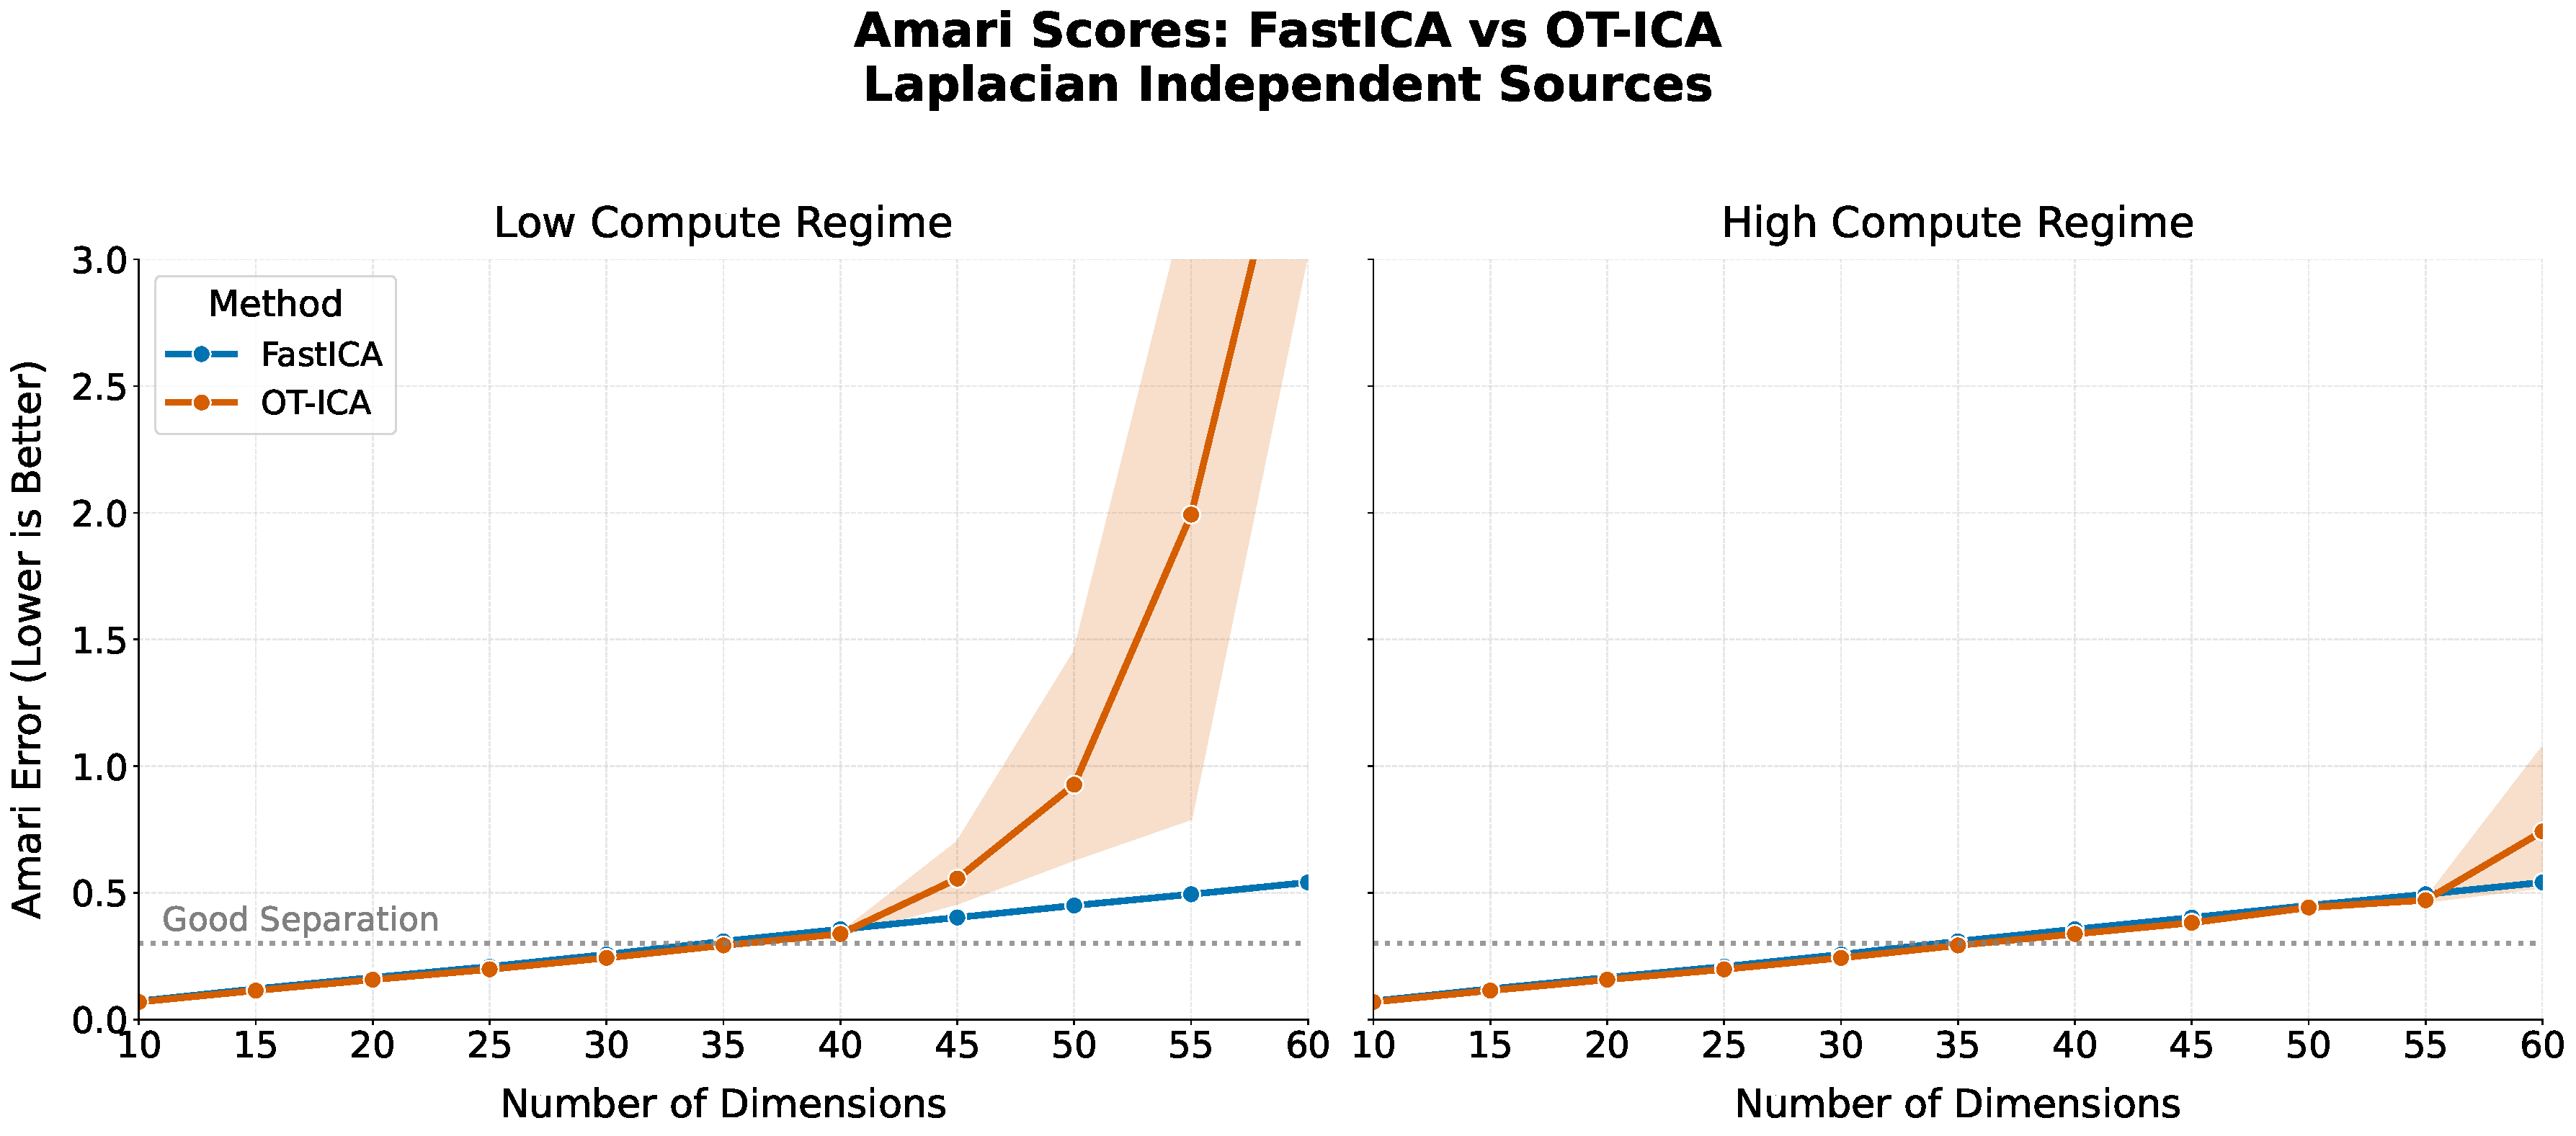
\includegraphics[width=0.83\textwidth]{laplace_amari_ot_ica_scaling.pdf}
    \caption{Amari error across dimensions for Laplacian sources at fixed $N=10{,}000$ samples. Both OT-ICA and FastICA hit 
    the same curse-of-dimensionality noise ceiling at $d=40$, a finite-sample sparsity effect shared by all empirical ICA methods at this regime.}
\end{figure}

While OT-ICA maintains error rates comparable to FastICA ($E < 0.3$) in lower dimensions, both algorithms exhibit a loss in unmixing quality at $d=40$. 
This limit is a manifestation of the curse of dimensionality. The expected error of the empirical Wasserstein distance scales as $\mathcal{O}(N^{-1/d})$. 
As $d$ grows, a fixed finite sample fails to densely populate the state space, creating massive empty regions that swallow the gradient signal.

\begin{figure}[htbp]
    \centering
    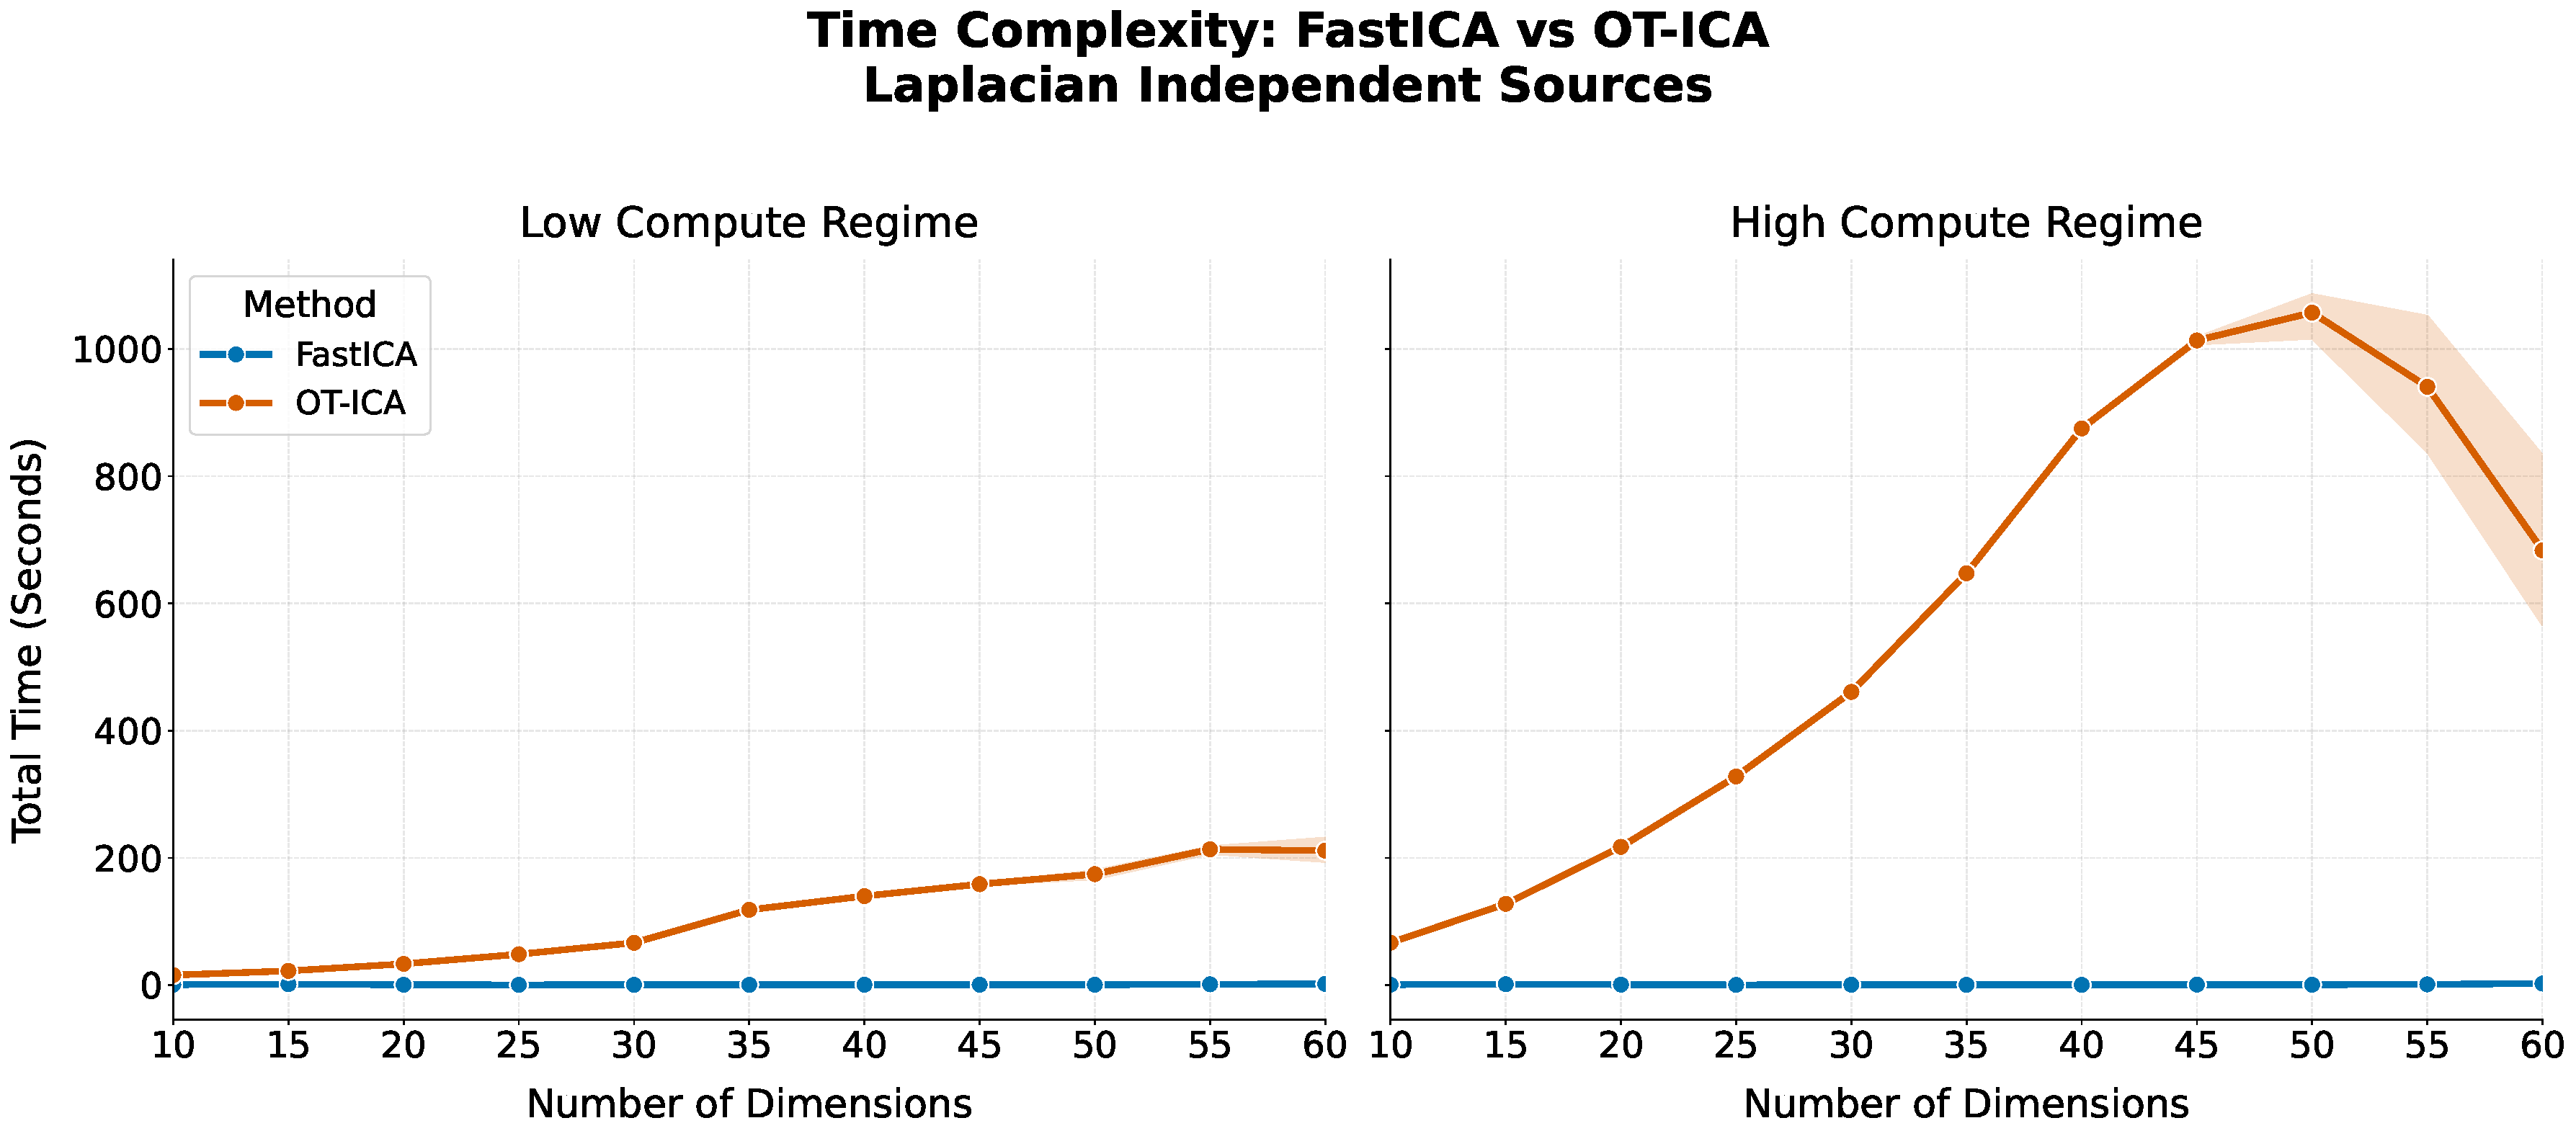
\includegraphics[width=0.83\textwidth]{laplace_time_ot_ica_scaling.pdf}
    \caption{Total execution time (in seconds) for FastICA and OT-ICA across dimensions.}
\end{figure}

The execution time for OT-ICA scales more steeply than FastICA. FastICA evaluates to $\mathcal{O}(d N)$ per iteration, making it computationally superior for exclusively homogeneous, continuous mixtures that do not trigger its proxy blind spots. OT-ICA incorporates parallel sorting across multiple restarts ($\mathcal{O}(K \cdot d N \log N)$), trading execution speed for reliability on complex topologies.

\section{Price Discovery Application: Data Generating Process and IS Definition}
\label{app:price_discovery}

\subsection{Data Generating Process}
We simulate a three-market VECM following the non-Gaussian information-share framework of \citet{zema2025}. The three markets share a single common efficient price, with long-run impact vector $\psi = (1, 1, 1)^\top$ (each market moves one-for-one with the common trend). The true structural mixing matrix is diagonal:
\begin{equation}
    \mathbf{B}_{\text{true}} = \mathrm{diag}\!\left(\sqrt{0.12},\, \sqrt{0.24},\, \sqrt{0.64}\right),
\end{equation}
which, as shown below, yields the target Information Shares $[0.12, 0.24, 0.64]$ by construction.

Structural innovations $\epsilon_t$ are drawn from Student-$t$ distributions with degrees of freedom $\nu_1 = 5$, $\nu_2 = 6$, $\nu_3 = 7$, normalized to unit variance. The VECM reduced-form residuals are $u_t = \mathbf{B}_{\text{true}}\,\epsilon_t$. Heavy tails are a realistic feature of high-frequency financial innovations and are what enables ICA identification: the non-Gaussianity of $u_t$ carries the rotation information that a Gaussian model would lose.

\subsection{Information Share Definition}
Under \citet{hasbrouck1995}, the Information Share of venue $i$ measures its contribution to price discovery:
\begin{equation}
    \mathrm{IS}_i = \frac{(\psi^\top \mathbf{B})_i^2}{\psi^\top \mathbf{B}\mathbf{B}^\top \psi}.
\end{equation}
With $\psi = (1,1,1)^\top$ and diagonal $\mathbf{B}_{\text{true}}$, the numerator equals $B_{ii}^2$ and the denominator equals $\sum_j B_{jj}^2 = 0.12 + 0.24 + 0.64 = 1$, so $\mathrm{IS}_i = B_{ii}^2 = \{0.12, 0.24, 0.64\}$.

\subsection{Estimation Procedure}
The reduced-form covariance is $\boldsymbol{\Omega} = \mathbf{B}\mathbf{B}^\top$. Cholesky or eigendecomposition of $\boldsymbol{\Omega}$ yields the whitening transform $\mathbf{S} = \boldsymbol{\Omega}^{1/2}$; the orthogonal rotation $\mathbf{C}$ satisfying $\mathbf{B} = \mathbf{S}\mathbf{C}$ is then identified from the non-Gaussianity of $\mathbf{S}^{-1}u_t$ by OT-ICA. In this simulation $\boldsymbol{\Omega}$ is treated as known; in practice it is estimated from VECM residuals by OLS. Two economic constraints are imposed post-estimation: the Hungarian algorithm \citep{kuhn1955hungarian} resolves the permutation ambiguity by assigning each structural shock to the market for which it explains maximum variance; sign normalization enforces a positive own-market impact. IS estimates are then computed from $\hat{\mathbf{B}} = \mathbf{S}\hat{\mathbf{C}}$ using the Hasbrouck formula above.

\section{EEG Application Details}
\label{app:eeg}

\subsection{Dataset and Preprocessing}
We use the MNE sample dataset (\texttt{sample\_audvis\_raw.fif}), a publicly available MEG/EEG recording with auditory and visual stimuli.
Five frontal EEG channels (EEG\,001--005) are extracted and cropped to a 10\,s segment (10--20\,s from onset).
A zero-phase FIR bandpass filter (1--40\,Hz, \texttt{firwin} design) is applied before ICA to remove DC drift and high-frequency noise.
Signals are then z-score normalized per channel: $\tilde{x}_i = (x_i - \mu_i)/\sigma_i$.

\subsection{OT-ICA Configuration}
Deflation phase: 50 random restarts, 200 iterations per restart, dither $\sigma = 0.01$.
Symmetric refinement phase: 400 gradient steps, learning rate $\eta = 0.05$, mini-batch size 512, dither $\sigma = 0.01$, symmetric decorrelation retraction.
No distributional assumptions are imposed; the algorithm operates on the 5-channel whitened signal.

\subsection{Artifact Identification and Evaluation}
Independent components are ranked by excess kurtosis $\kappa = \mathbb{E}[(z - \mu)^4]/\sigma^4 - 3$.
The component with the highest $\kappa$ is designated the ocular artifact; blink artifacts are impulsive (super-Gaussian) and are expected to dominate on frontal channels.
Reconstruction quality is evaluated as the RMS amplitude reduction in a $\pm$250\,ms window around the maximum-amplitude blink event, computed as:
\begin{equation}
    \text{RMS reduction} = 1 - \frac{\|\mathbf{x}_{\text{clean}}\|_{\text{RMS}}}{\|\mathbf{x}_{\text{raw}}\|_{\text{RMS}}}.
\end{equation}
The cleaned signal is obtained by zeroing the artifact component in the ICA source space and applying the inverse total unmixing matrix $(\mathbf{W}_{\text{eeg}} \, \mathbf{W}_{\text{white}})^{-1}$.

\end{document}